\section{Mechanical Design and Enclosure}
\label{sec:mechanical_design}

\subsection{Manufacturing Technologies and Materials}
\label{subsec:manufacturing_tech}
The mechanical construction of the RLCV3 system relies on a combination of additive manufacturing, standardized metal components, and specialized fastening techniques to achieve a robust and professional assembly.

\subsubsection{Additive Manufacturing (3D Printing)}
The fabrication of custom enclosures, structural brackets, and end caps is performed using \ac{FDM}.
A BambuLab X1C printer, equipped with a textured \ac{PEI} build plate, is utilized to ensure consistent adhesion and a high-quality surface finish.\\ 

Two primary thermoplastic filaments are employed based on the functional requirements of the components:
\begin{itemize}
	\item \textbf{BambuLab PLA-Basic}: This material is used for the majority of the structural parts, including the main PCB enclosures, as well as the housing components for the Spotlight and Panel variants \cite{inet:bambulab_pla}.
	It offers a favorable balance of rigidity and dimensional accuracy.
	\item \textbf{BambuLab PLA-CF}: A Carbon Fiber reinforced \ac{PLA} composite is utilized for the tube light end caps \cite{inet:bambulab_placf}.
	The addition of carbon fiber enhances the stiffness of the parts and provides a distinctive matte surface finish, contributing to the aesthetic quality of the visible components.
\end{itemize}

To ensure mechanical integrity, specific print parameters are strictly adhered to.
Components are fabricated using a 0.4 mm nozzle with a layer height of 0.12 mm, allowing for fine detail resolution.
Structural strength is prioritized through the use of increased wall thickness rather than high infill density.
Parts are typically sliced with 3 to 4 wall perimeters and 2 to 3 top and bottom layers.
The infill density is set between 20\% and 30\%, utilizing 3D-honeycomb or cubic patterns to provide isotropic strength distribution.
Components subjected to higher mechanical stress, such as the connector systems detailed in section \ref{subsec:connection_systems}, are designed with significantly thicker walls to withstand operational loads.

\subsubsection{Fastening Technology}
To ensure durability and serviceability, the assembly avoids the use of direct threading into plastic or loose nuts.
Instead, brass threaded inserts (typically M3) are integrated into the 3D-printed components.
These inserts are installed using a heat-set process, where a soldering iron is used to melt the plastic locally, allowing the knurled insert to sink into the part and bond securely upon cooling.
This method provides medium pull-out resistance and torque capability \cite{inet:cnckitchen_inserts}.
Furthermore, it simplifies the assembly process by eliminating the need for a counter-wrench and allows for repeated disassembly without degrading the fastening interface.

\subsubsection{Aluminum Extrusion Profiles}
The core structure of the light tube variants is formed by an extruded aluminum U-profile \cite{inet:alu_profile_amazon}.
This profile serves a dual purpose: it acts as the rigid chassis for the fixture and functions as a passive heatsink for the LED strips \cite{inet:alu6063_properties}.
The selected profile features a width of approximately 27 mm and a height of 12 mm.
Originally supplied in 2-meter lengths, the profiles are cut to 1 meter.
Light diffusion is achieved via a compatible milky-white diffuser cover, which snaps into the profile and adds 13 mm to the total height.
Although specific manufacturer data regarding the thermal resistance and structural modulus of this profile is unavailable, empirical testing has confirmed its suitability for dissipating the thermal load generated by the LEDs in this application.
The precise dimensions provided by the manufacturer, as well as the profile cross-section, can be seen in figure \ref{fig:aluprofileedgy}.

\begin{figure}[H]
	\centering
	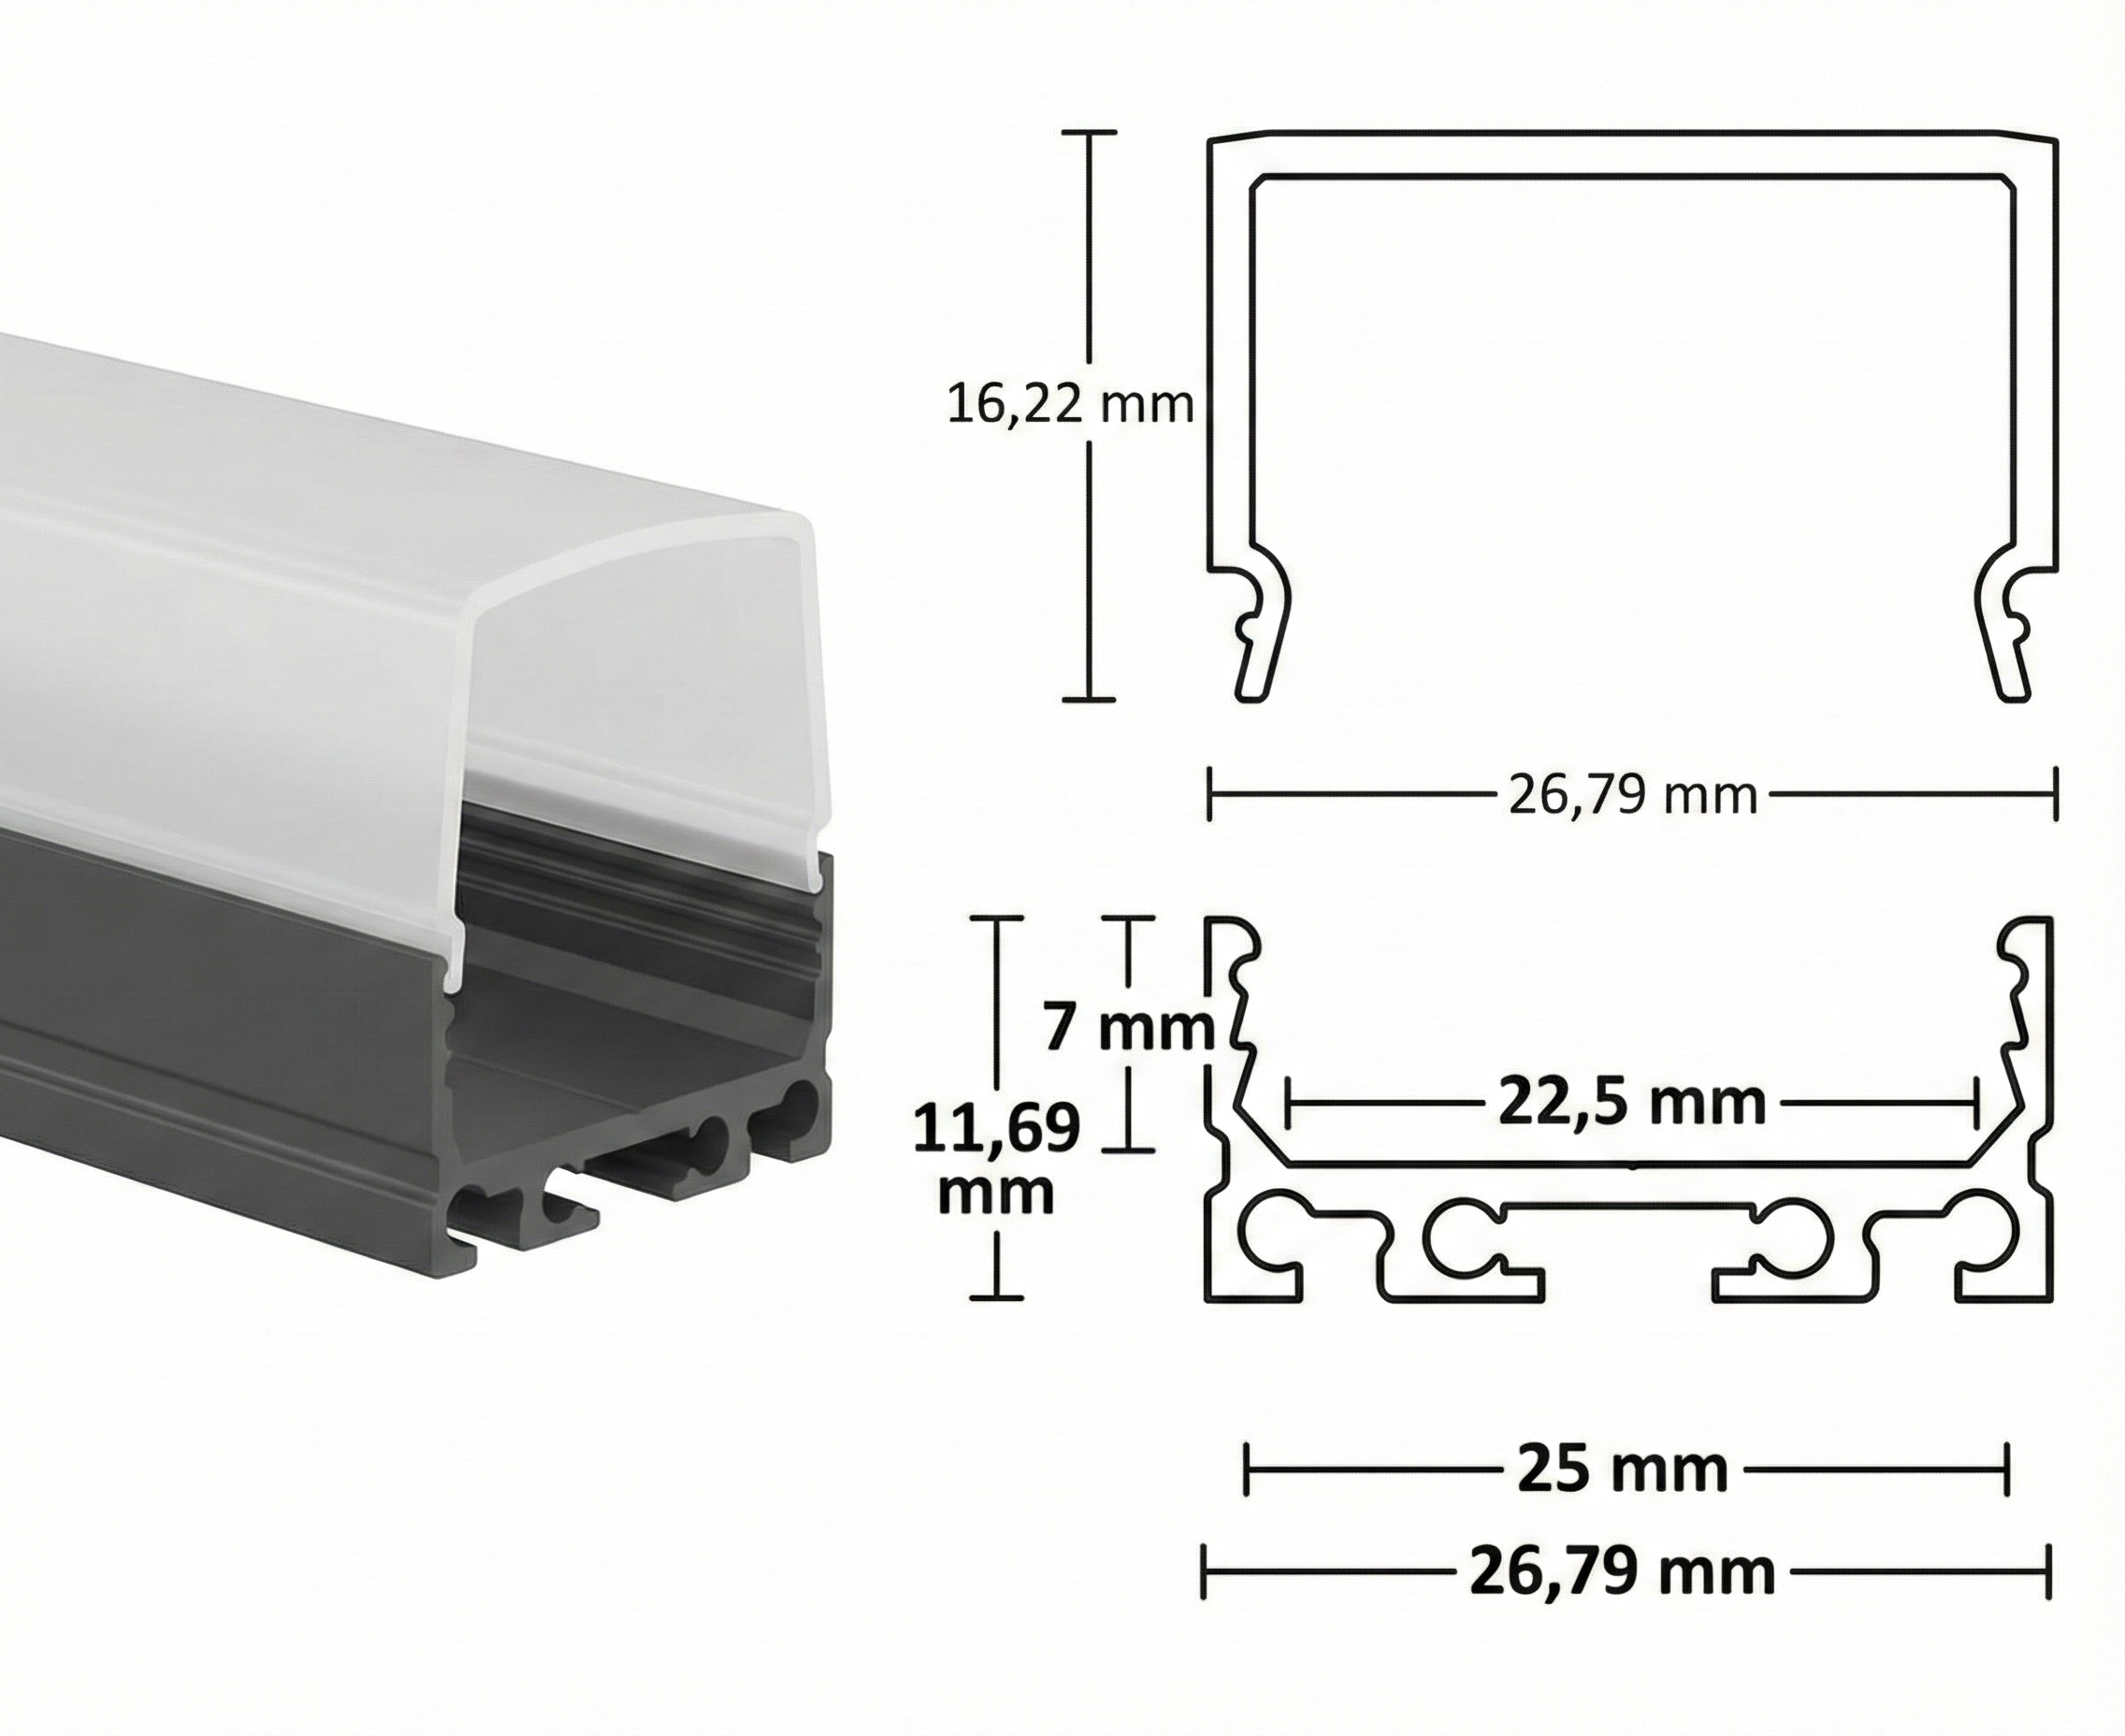
\includegraphics[width=0.6\linewidth]{graphics/alu_profile_edgy}
	\caption{Cross-section of the aluminum U-profile used for the tube light structure.}
	\label{fig:aluprofileedgy}
\end{figure}

\subsection{Light Tube Enclosures}
\label{subsec:light_tube_enclosures}
	Holes are drilled through the aluminum profile, and screws are inserted from the inside channel (the surface to which the \ac{LED} strip is adhered).
	These screws engage with the threaded inserts installed in the 3D-printed parts.
	This approach ensures a clean exterior finish with no visible screw heads on the printed parts and provides a secure mechanical connection.
	Typically, each major component is secured with four screws to prevent rotation and ensure structural rigidity.

\subsubsection{Variant V2 (MOSFET)}
\label{subsubsec:light_tube_v2}
In the V2 iteration, the mechanical design integrated the controller housing directly into one of the end caps.
This single-piece assembly served as both the termination for the tube and the enclosure for the \ac{PCB}.
Mechanical mounting for the fixture was provided via a standard tripod screw thread embedded in the housing.
However, this design lacked the modularity required for more advanced mounting scenarios.
Consequently, this mechanical configuration is considered deprecated.
The V2 electronic hardware is compatible with the improved V3 mechanical design, and therefore, no further development is being conducted on the specific V2 enclosure geometry.

\subsubsection{Variant V3 (Addressable)}
\label{subsubsec:light_tube_v3}
The V3 design represents the current standard for the light tube fixtures, featuring a more modular and robust architecture.
The assembly consists of distinct end caps at both the top and bottom of the tube, which incorporate mechanical interfaces for the connector systems.\\

The controller electronics are housed in a dedicated, two-part enclosure mounted along the length of the profile, rather than at the end.
This enclosure comprises a base plate, which is bolted to the aluminum profile and supports the \ac{PCB}, and a removable lid.
The lid protects the electronics while providing necessary apertures for the \ac{OLED} display, input connectors, and the rotary encoder.\\

Electrical connection between the external controller and the internal \ac{LED} strip is achieved by routing three separate cables through drilled holes into the profile's interior.
To facilitate precise assembly, a 3D-printed drill template is available, allowing the user to accurately mark all 14 required holes: 12 for mechanical fastening of the components and 2 for wire feed-throughs.
Inside the profile, a specialized clip is used to secure the data wire.
This clip is designed to be held in place by the adhesive backing of the \ac{LED} strip itself, ensuring the internal wiring remains unobtrusive and does not cast shadows on the diffuser.\\

\subsection{Panel Enclosure}
\label{subsec:panel_enclosure}
The enclosure for the Panel Light variant is constructed around a central structural component, referred to as the main body.
This part serves as the mounting interface for the electronic subsystems, with the \ac{LED} driver \ac{PCB}s positioned on the front face and the main control unit secured to the rear. \\

Electrical connectivity between the rear-mounted controller and the front-facing \ac{LED} modules is established via four wires (carrying power and \ac{I2C} signals), which are routed through a dedicated feed-through channel within the main body.
The lighting array consists of five distinct segments, each managed by its own driver \ac{PCB} mounted on the front.\\

Thermal management is addressed by a cooling fan located at the rear, which is enclosed by a protective lid.
Similarly, the \ac{LED} driver \ac{PCB}s on the front and the main control \ac{PCB} on the back are shielded by their respective covers to ensure safety and prevent accidental contact.\\ 

For positioning and mounting, the assembly features a U-shaped frame.
This frame allows for tilt adjustment and attachment to a standard tripod, secured using an M8 bolt and a wing nut for tool-free adjustment.
Additionally, the design accommodates a diffuser, which can be mounted in conjunction with the U-frame to soften the light output.

\subsection{Spotlight Enclosure}
\label{subsec:spotlight_enclosure}
The mechanical design of the Spotlight variant is centered around a high-performance aluminum heatsink equipped with an active cooling fan, essential for dissipating the heat generated by the high-power \ac{COB} \ac{LED}.\\

The main enclosure body wraps around this heatsink and forms the front face of the fixture.
It features a central aperture designed to accommodate a $60^{\circ}$ lens, which directs the light output.
Internally, a specialized diffusion cube, printed from transparent \ac{PETG} \cite{inet:bambulab_petg}, is positioned between the \ac{LED} and the lens.
This component is critical for blending the distinct red, green, and blue zones of the \ac{COB} \ac{LED} to ensure a uniform color mixture before the light passes through the lens.\\

The control \ac{PCB} is mounted directly to the main body.
A dedicated lid covers the electronics, providing necessary cutouts for peripheral connections and user interface elements.
Similar to the Panel variant, the Spotlight utilizes a U-shaped mounting frame.
This frame facilitates tilt adjustment and tripod mounting, secured via an M8 bolt and a wing nut, allowing for flexible positioning in various lighting setups.

\subsection{Connection Systems}
\label{subsec:connection_systems}
The system features two distinct connection methods designed to address different use cases, ranging from rapid, temporary mounting to robust, structural assembly.

\subsubsection{System \enquote{click \& hope}}
The \enquote{click \& hope} system is a friction-fit mounting solution designed to engage with the external longitudinal grooves of the aluminum profile.
Due to this specific mechanical interface, it is exclusively compatible with the light tube variants.
The primary advantage of this system is the speed of assembly, allowing for the quick attachment of accessories such as tripod mounts.
These mounts typically integrate a threaded insert to interface with standard photography equipment and feature a rosette coupling to enable discrete rotational adjustment. \\

Despite its convenience, the system relies on the clamping force of the printed parts against the profile grooves.
Consequently, it is less structurally secure than bolted connections.
While a spacing bracket for aligning multiple tubes has been prototyped, the ecosystem for this mounting standard is limited.
Due to the superior reliability of the end-cap-based mounting system, further development of this clip-on mechanism is currently not planned.

\subsubsection{System \enquote{screw it!}}
In contrast to the friction-based approach, the \enquote{screw it!} system offers a robust, mechanical interlocking connection.
This system utilizes the structural hardpoints integrated into the end caps of the V3 light tube variants to facilitate the creation of complex, multi-fixture arrays.\\

A comprehensive suite of modular connector components has been developed to support various geometric configurations, including linear couplers, T-pieces, and cross-connectors.
For free-standing applications, specialized feet are utilized.
These feet consist of 3D-printed shells filled with plaster to provide the necessary ballast.
A key maintenance feature of the feet is the detachable mounting adapter; this design allows for the replacement of the mechanical interface in the event of damage without requiring the disposal of the entire weighted base. \\

Assembly is achieved by inserting screws from the rear of the connector components, which engage with the threaded inserts in the tube end caps.
To ensure a seamless appearance and structural rigidity, a clamping mechanism can be applied from the front.
This clamp actively pulls the connected tubes towards the central connector hub, minimizing gaps and preventing rotation.
Figure \ref{fig:crossconnectorclamp} illustrates this assembly from a side perspective to demonstrate the interconnection of parts; for clarity, the end caps are rendered in green, the cross-connector in blue, and the clamping mechanism in red.
Technical drawings detailing the dimensions and tolerances of this interface are provided in appendix~\ref{sec:cad_models} \nameref{sec:cad_models}.

\begin{figure}[H]
	\centering
	\includegraphics[width=0.7\linewidth]{graphics/cross_connector_clamp}
	\caption{Cross connector with two end caps and clamp mechanism.}
	\label{fig:crossconnectorclamp}
\end{figure}